\documentclass{article}

\usepackage{amssymb}
\usepackage{amsfonts}
\usepackage[tbtags]{amsmath}
\usepackage{amscd}
\usepackage{amsthm}			% Продвинутая математика
\usepackage{mathtext}
\usepackage{cmap}
\usepackage[T2A]{fontenc}
\usepackage[utf8]{inputenc}			% cp1251
\usepackage[english, russian]{babel}
%\usepackage{literat}
\usepackage{pifont}
\usepackage{bm}
\usepackage{array}			% Ширина столбиков в массиве
\usepackage{dcolumn}
\usepackage{hhline}
\usepackage{multirow}
\usepackage{graphicx}
\usepackage{rotating}
\usepackage{calc}
\usepackage{tabularx}
\usepackage{afterpage}
\usepackage{ifthen}
\usepackage{caption2}
\usepackage{substr}
\usepackage[mathscr]{eucal}  %% My addition
\usepackage{mathrsfs}        %% My addition
\usepackage{hypbmsec}        %% My addition
\usepackage{latexsym}        %% My addition
\usepackage{xypic}           %% My addition
\RequirePackage{soul}
\RequirePackage{verbatim}    %% My addition
\RequirePackage{chapterbib}
\RequirePackage{enumerate}

\usepackage[shortcuts]{extdash}
\usepackage{ragged2e}
\usepackage{etoolbox}
\usepackage{lipsum}

%\usepackage{flafter}
\usepackage[section,above,below]{placeins}

\usepackage{indentfirst}
\usepackage[a4paper, top=20mm, left=30mm, right=20mm, bottom=25mm]{geometry}

\title{Исследование прогнозных своиств решения обратной задачи идетификации модели аквифера для нефтяного месторождения}
\author{V.P. Kosyakov}


\begin{document}
	\maketitle
	\textbf{Abstract}. При моделировании разработки нефтяного месторождения одним из важнейших шагов является решение обратной задачи, решение которой, как правило, заключается в подборе параметров модели для наилучшей настройки на историю разработки. Однако целью моделирования является не только повторение показателей разработки на историческом периоде, но и получение достоверного прогноза поведения моделируемого объекта в будущем. Поэтому с точки зрения долгосрочных прогнозных характеристик модели необходимо выполнение не только параметрической, но и структурной идентификации модели.
В данной работе на примере решения задачи структурно-параметрической идентификации модели водоносного контура (аквифера) для моделирования разработки нефтяного месторождения проведено исследование их прогнозных характеристик. Показано, что в результате выполнения структурно-параметрической идентификации модели ее прогнозные свойства могут быть существенно улучшены по сравнению со случаем обычной параметрической идентификации. 

\textbf{Keywords}: обратная задача, структурно-параметрическая идентификация, моделирование, аквифер
\section{INTRODUCTION}
	В процессе моделирования разработки нефтяного месторождения одним из важнейших шагов является решение обратной задачи. Решение которой, как правило, заключается в подборе параметров модели для наилучшей настройки на историю разработки. В свою очередь, целью моделирования является не только повторение показателей разработки на историческом периоде, но и получение достоверного прогноза поведения моделируемого объекта. Выбор математической модели определяется целями и задачами, для решения которых она будет использована. В рассматриваемом случае целью является получение качественного прогноза. Исходя из требований задач адаптации и прогнозирования, задача идентификации заключается в определении структуры и параметров математической модели, обеспечивающих удовлетворительное описание исторических данных и имеющих наилучшее прогнозные характеристики.
	
	Для оценки прогнозных характеристик модели часто используют разбиение исторического периода на 2 временных интервала: на первом производят адаптацию модели, на втором валидацию - оценку прогнозных свойств модели. В работе \cite{mus} было показано, что наилучшая адаптация не обязательно имеет наилучшие прогнозные свойства, которые в значительной степени зависят от сложности выбранной модели. Кроме того прогнозные характеристики зависят от конкретных условий (управляющих параметров) работы модели на этапах адаптации и валидации.
	
	В настоящей работе представлено исследование зависимости прогнозных характеристик модели от согласованности режимов работы на этапах адаптации и валидации. На примере задачи идентификации модели водоносного горизонта и адаптации его параметров для нефтяного месторождения, показана важность структурной идентификации с точки зрения долгосрочных прогнозных характеристик модели. В качестве прогнозируемого параметры выступает пластовое давление, характеризующее “энергетический” потенциал залежи.  Модель водоносного контура важна для прогнозных характеристик модели с точки зрения его энергетического состояния в условиях интенсивной разработки месторождения \cite{kos}, к которой можно отнести эксплуатацию в режиме истощения, разбуривание новых скважин, формирование системы поддержания пластового давления, массированную остановку скважин и т.д. 

\section{MODEL}
Для решения поставленной задачи в качестве фильтрационной модели использовалась двумерная математическая модель однофазной фильтрации для слабо сжимаемой жидкости \cite{bas}. Для моделирования поведения водоносного контура использовался набор из 4-х моделей разной степени сложности \cite{dake},\cite{fet}. Сложность модели определяется количеством настраиваемых параметров. Обозначим через $F(P_{aq}, P,\nu)$ - функцию описывающую приток жидкости, которая в общем случае завист от средгнегно давления в аквифере $P_{aq}$, давления в расчётной области $P$ и от вектора параметров $\nu$. Исследование прводилось для четырёх моделей водоносного горизонта:
\begin{enumerate}
\item модель позволяющая описать поведение изолированного объекта, нет адаптируемых параметров (M1);
\item модель постоянного давления на контуре питания (аквифер бесконечного объёма), имеет один настраиваемый параметр (M2);
\item модель аквифера конечного объёма, имеет 2 настраиваемых параметра (M3); 
\item модель аквифера конечного объёма с удаленным контуром питания - 3 настраиваемых параметра (M4).
\end{enumerate}
Таким образом систему уравнений можно записать в следующем виде:
\begin{equation} \label{fil}
\left\{\begin{array}{crl}
\triangledown\sigma\triangledown P = \beta^*h\frac{dP}{dt}+\delta(x,y)\\
q_{aq} = F(P,\nu)
\end{array}\right.
\end{equation}

\begin{equation} \label{bc}
\delta(x,y)  = \left\{\begin{array}{crl}
0\;при\;(x,y) \notin\ \Gamma_{in}\cup\Gamma_{out}\\
q_j\;при\;(x,y) \in \Gamma_{in}\\
q_{aq}\;при\;(x,y) \in \Gamma_{out}
\end{array}\right.
\end{equation}
\begin{equation*}
P(t=0) = P_{aq}(t=0) = P_0
\end{equation*}
где $\sigma$ - гидропроводность, $P$ - пластовое давление, $\beta^*$ - эффективная сжимаемость, $h$ - эффективная толщина, $q_j$ - расход жидкости в $j$ скважине, $\Gamma_{in}$ - множество координат источников/стоков (скважин), $\Gamma_{out}$ - внешняя граница, $P_0$ - пластовое давление в начальный момент времени $t=0$.

Модели водоносного контура (M1-M4) можно описать следкющими уравнениями:
\begin{equation}
q_{aq}=0
\end{equation}
\begin{equation}
q_{aq} = \lambda\sigma(P|_{\Gamma_{out}}-P_c)
\end{equation}
\begin{equation}
\beta^*V_{aq}\frac{dP_{aq}}{dt} = \lambda\oint_{\Gamma_{out}}\frac{\sigma}{h}(P-P_{aq})d\Gamma_{out}
\end{equation}
\begin{equation}
\beta^*V_{aq}\frac{dP_{aq}}{dt} =\lambda\oint_{\Gamma_{out}}\frac{\sigma}{h}(P-P_{aq})d\Gamma_{out} + \kappa(P_{aq}-P_c)
\end{equation}
где $V_{aq}$ - объём аквифера, $P_с$ - давление на контуре питания ($P_c = P_0$), $P_{aq}$ - давление в аквифере, $\lambda$ - коэфициент продуктивности аквифера, $\kappa$ - продуктивность удалённой зоны. Таким образом вектор $\nu = [\lambda, V_{aq}, \kappa]$, для модели аквифера M4.

При испрользовании (\ref{fil} - \ref{bc}) решается обратная задача, которая заключается в  минимизации целевой функции $J$, в качестве который выступает MAPE (mean absolute percentage error). Аргументами целевой функции выступают фактические и расчётные значения пластового давления в точках расположения скважин. Целевая функция записывается следующим образом:
\begin{equation} \label{mape}
J=\frac{1}{N}\sum_{i=1}^N{\left\vert\frac{p_c^i-p_f^i}{p_f^i}\right\vert}\rightarrow min
\end{equation}
где $p_c$ -расчетное значение пластового давления, $p_f$ - фактическое значение, $N$ - общее количество замеров. Решение задачи находится при использовании градиентного оптимизационного алгоритма и заключается в определении набора параметров модели соответствующих минимуму $J$ и удавлетворяющих ограничениям в виде неравенства: $\nu_{min}\leq\nu\leq\nu_{max}$.

В фильтрационную модель был введён настраиваемый параметр $a$ - множитель на гидропроводность, таким образом в (\ref{fil}) $\sigma = a\cdot\sigma_0$, где $\sigma_0$ - начальное приближение для гидропроводности, $a>0$. Следовательно для решения задачи адаптации необходимо будет определить значения вектора параметров $u = [a, \nu]$ длинной от 1 до 4. Значение градиента целевой функции для компонент можно записать в следующем виде:

\begin{equation}
\frac{dJ}{du} = \frac{1}{N}\sum_{i=1}^N sgn\left(\frac{p_c^i-p_f^i}{p_f^i}\right)\frac{dp_c^i}{du}
\end{equation}
Таким образом для решения обратной задачи необходимо чтобы
\begin{equation} \label{rp}
	 \frac{dJ}{du} \rightarrow 0
\end{equation}
Решение прямой (\ref{fil}-\ref{bc}) и обратной (\ref{rp}) задачи находилось численно в неявном виде 
при использвании двумерной неструктурированной сетки.

\section{CALCULATION}
В качестве примера, была решена обратная задача структурно-параметрической идентификации для нефтяного месторождения. Для решения задачи необходим набор данных (размеры расчётной области, расположение скважин и показателей разработки по скважинам: расходы жидкости и давления), который был получен при помощи синтетической гидродинамической модели. Эти данные выступали в качестве "фактических" значений. 

Схема расположения скважин и условные обозначения представлены на рисунке \ref{fig:map}. 
%\center{
\includegraphics[height=6pc]{fig1.png}}
\begin{figure}
    \begin{minipage}[h]{0.69\linewidth}
      \center{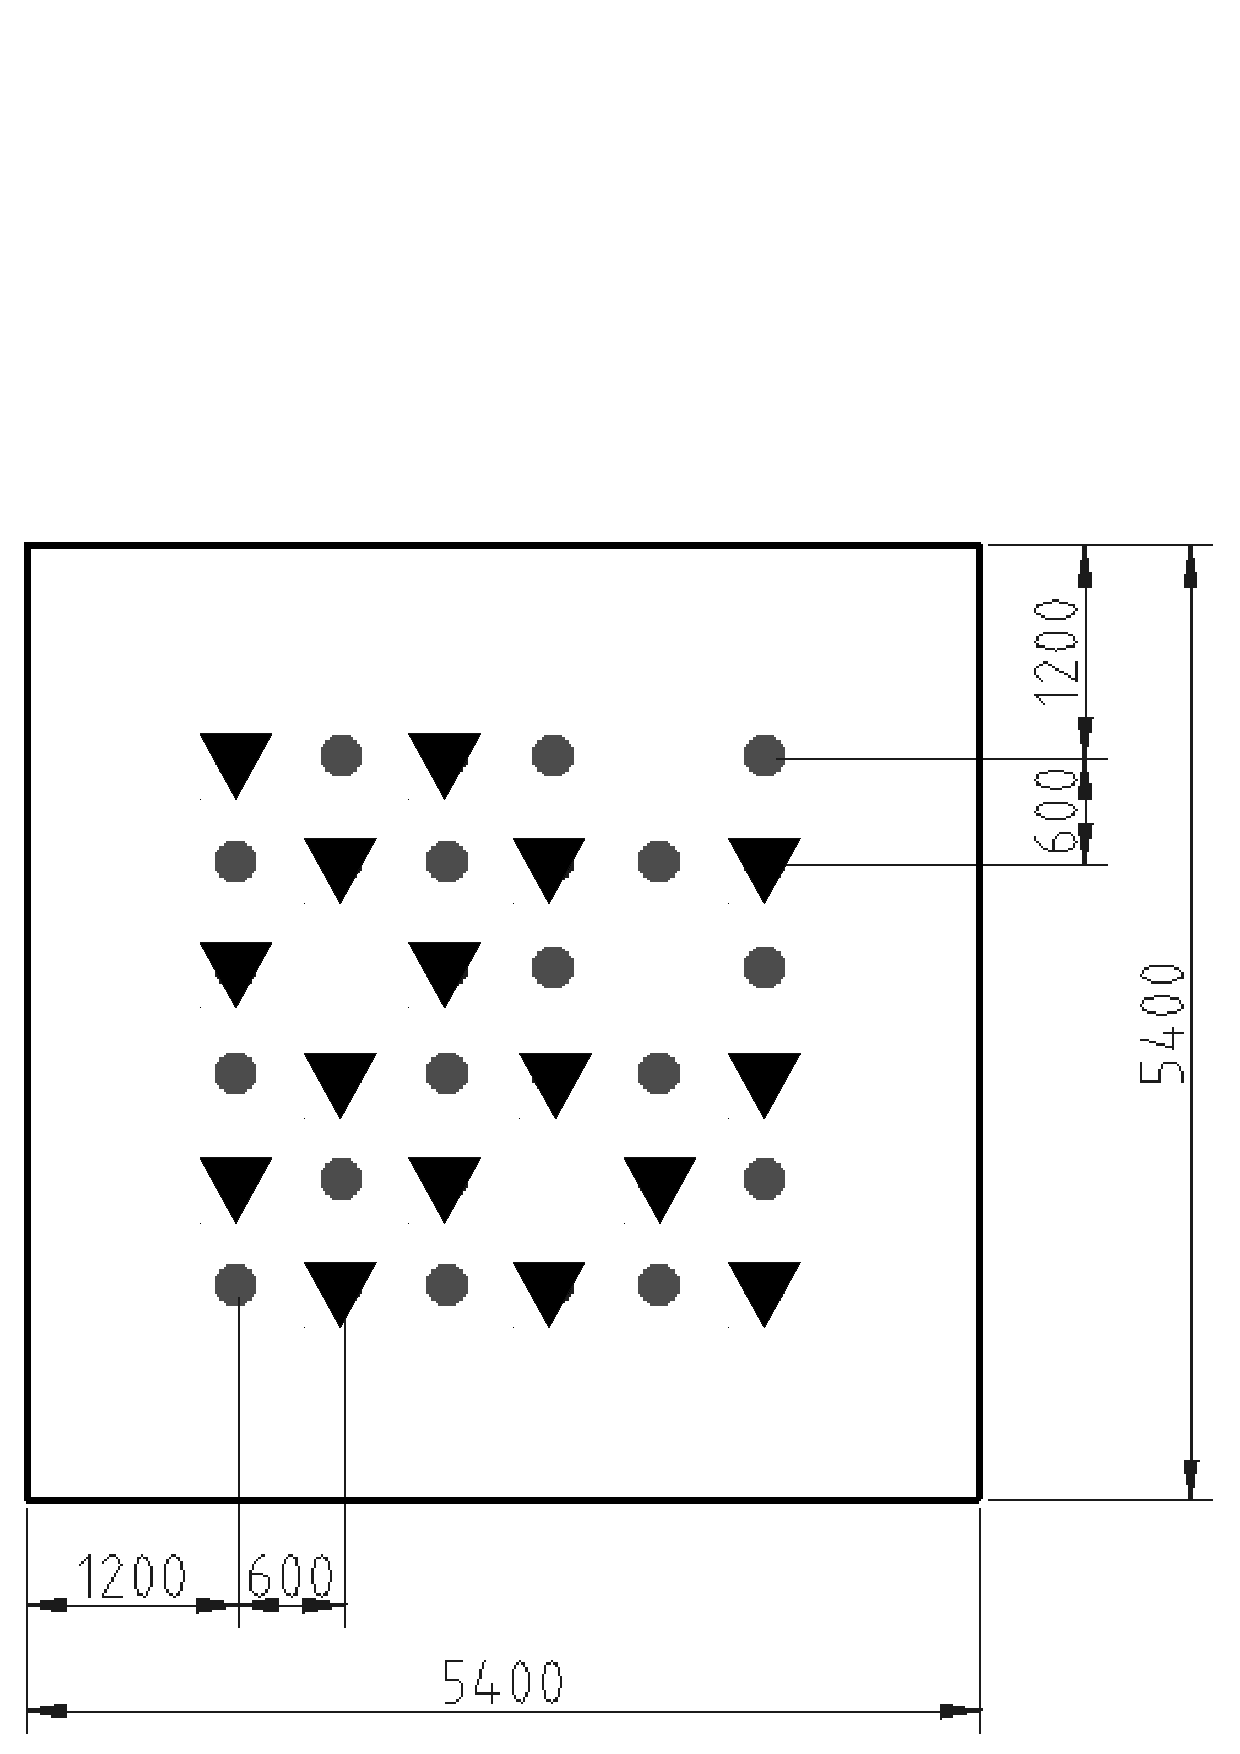
\includegraphics[width=16pc]{fig1a.png} \\ (a)}
    \end{minipage} \hfill
    \begin{minipage}[h]{0.29\linewidth}
      \center{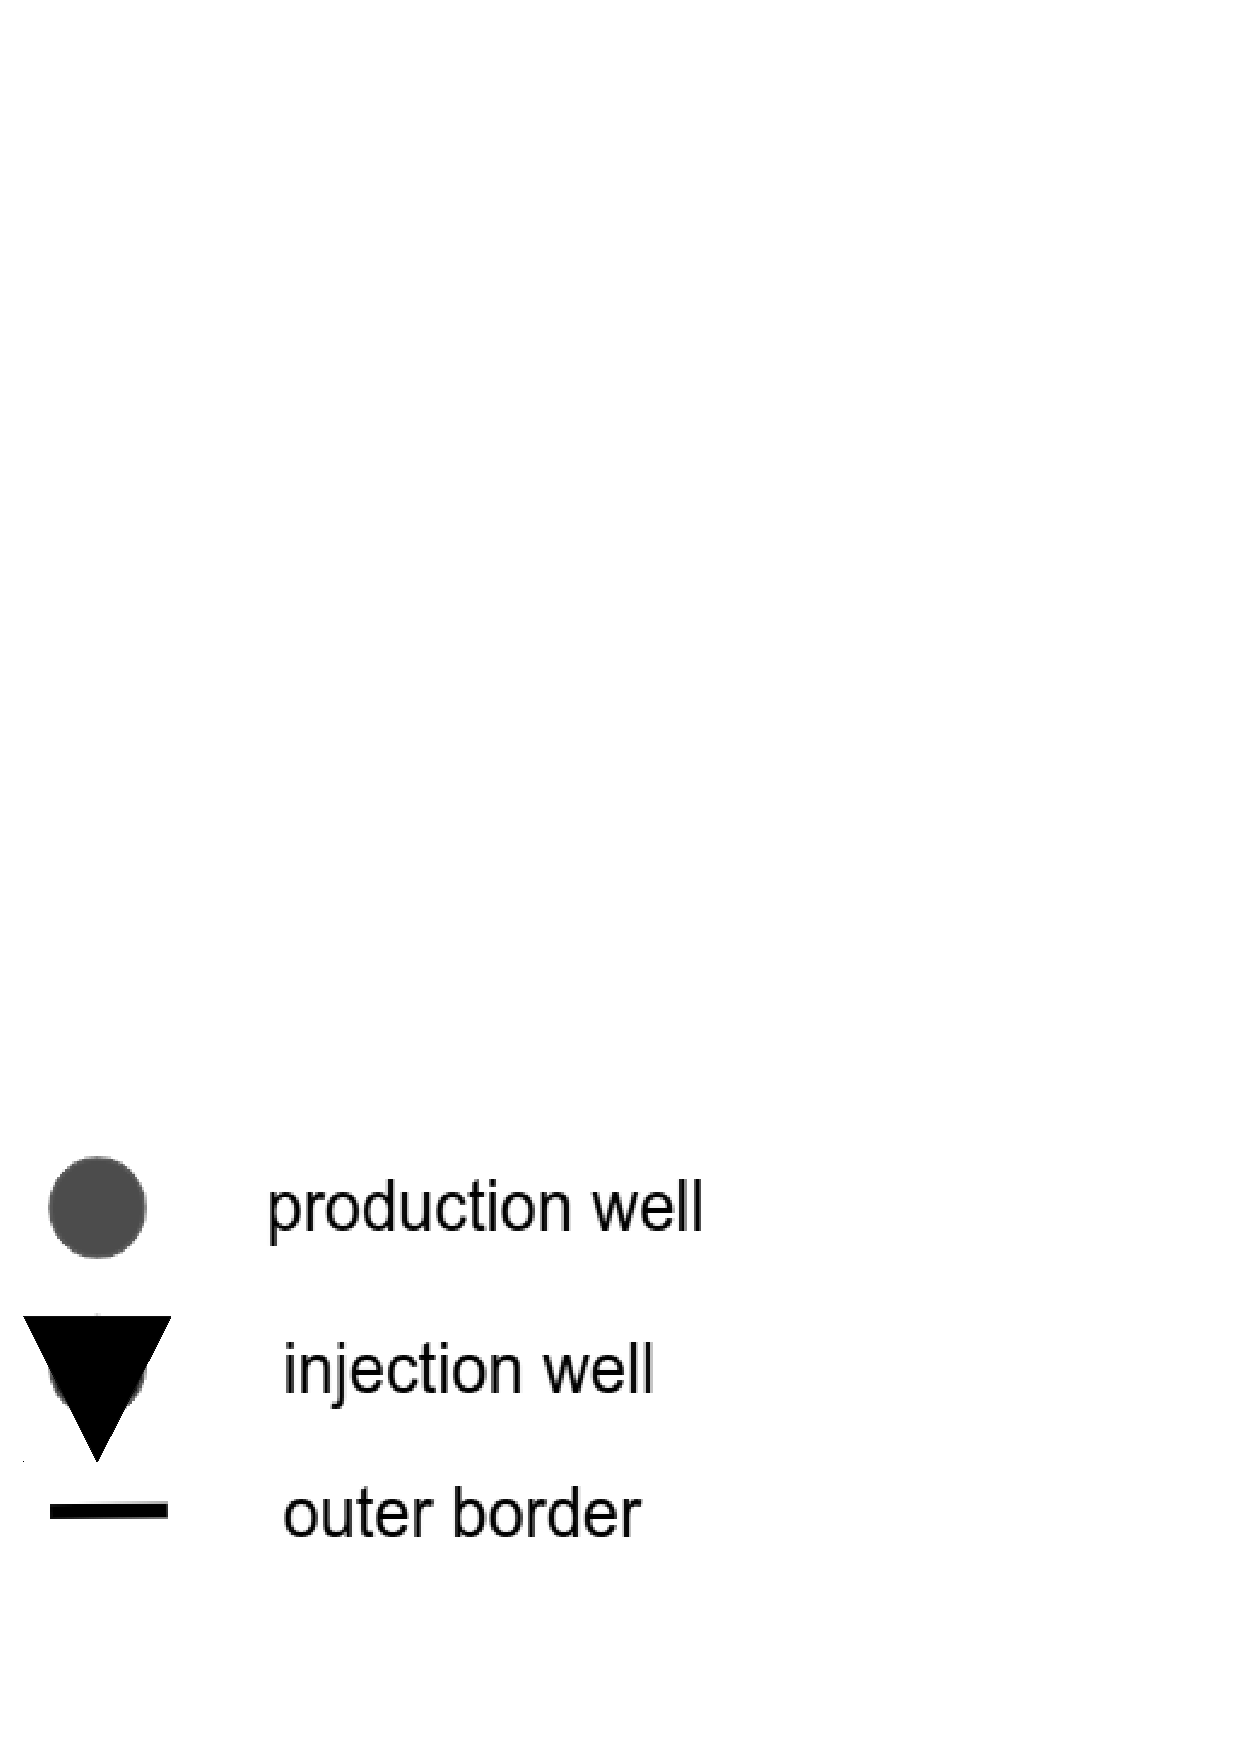
\includegraphics[width=8pc]{fig1b.png} \\ (b)}
    \end{minipage} 
    \caption{Схематическое представление расчётной области (a) и условные обозначения (b).}
    \label{fig:map}
\end{figure}
Месторождение разрабатывается при помощи 16 добывающих и 16 нагнетательных скважин. Период разработки составляет 10 лет, контур питаний был “подключён” по периметру расчетной области. Для решения задачи структурно-парамтерической идентификации временной интервал был разбит на 3 части по 72, 24 и 24 месяца соответсвенно:
\begin{enumerate}
\item с 01-2000 по 12-2005  период адаптации;
\item с 01-2006 по 12-2007  период валидации;
\item с 01-2008 по 12-2009  период прогноза.
\end{enumerate}
На временном интервале адаптации решается обратная задача для всех 4-х моделей, находяся неизветные параметры. На интервале валидации оцениваются прогнозные характеристики настроенной модели, и осуществляется выбор модели обладающей наилучшими прогнозными характеристиками. Дополнительно был выделен 3-й интервал - интервал прогноза, на котором производится оценка поведения адаптированной модели при значительном изменении управляющих параметров. Временной интервал для этапа адаптации  выбирался таким образом, чтобы он включал в себя поэтапный ввод всех скважин и был достигнут стационарный режим эксплуотации. Этап валидации также включает в себя интервал стационарной работы месторождения. 

Для этапа прогнозирования было рассчитано 3 сценария эксплуатации для каждой модели, и произведено сопоставление поведение основных параметров разработки. В качестве сценариев были расчитаны: S0 - стационарный режим работы, S1 - двукратное сокращение объёма нагнетаемой жидкости и S2 - двукратное увеличение объёма нагнетаемой жидкости по сравнению со сценарием S0. 

На рисунке \ref{fig:2din} представлена динамика среднего пластового давления для фактических данных (B - базовый вариант) и всех моделей водоносного горизонта (M1-M4 модели аквифера). На гистограмме \ref{fig:hist} показанны значения (\ref{mape}) для интервалов адаптации (adp) и валидации (val).
\begin{figure} 
    \begin{minipage}[h]{0.48\linewidth}
      \center{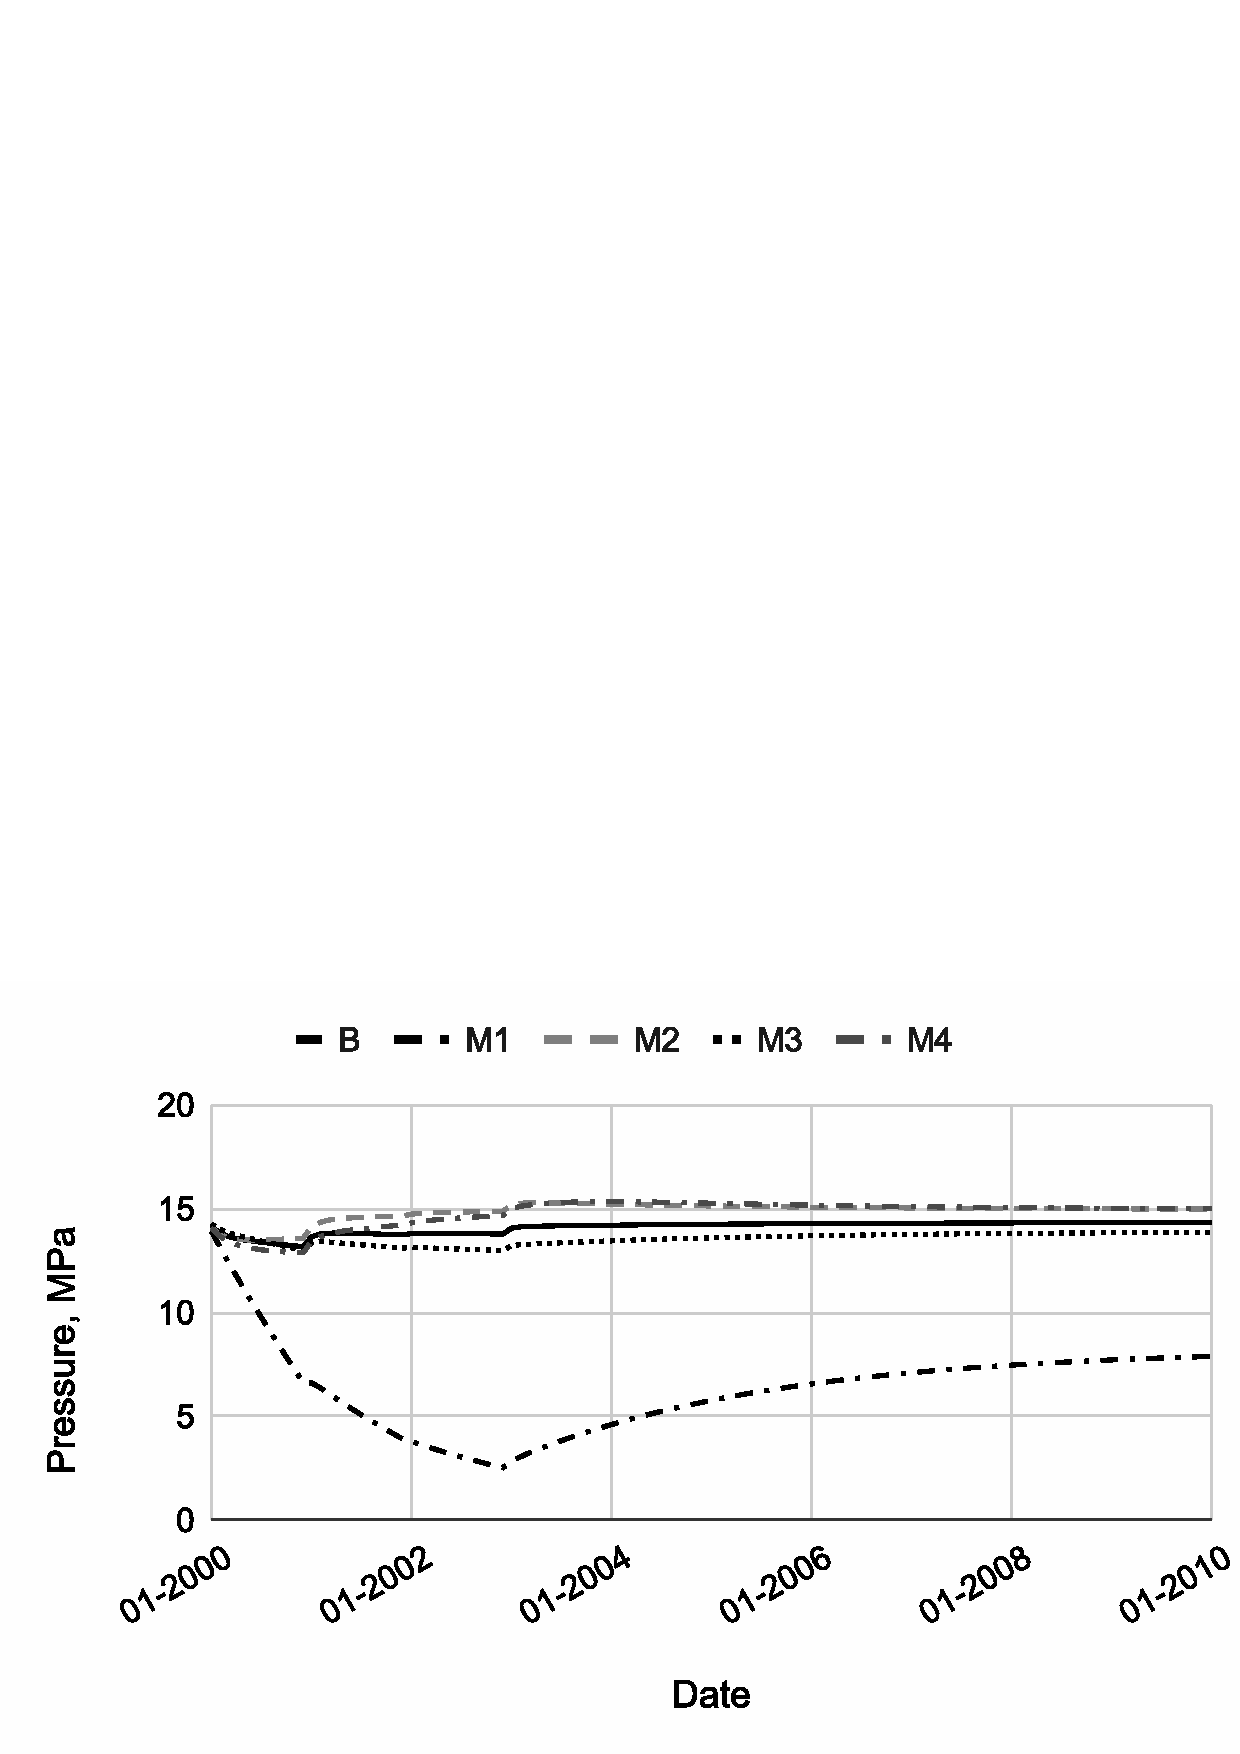
\includegraphics[height=0.65\linewidth]{fig2.png}}
      \caption{Динамика среднего пластового давления при разных моделях водоносного горизонта}
      \label{fig:din}
    \end{minipage} \hfill
    \begin{minipage}[h]{0.48\linewidth}
      \center{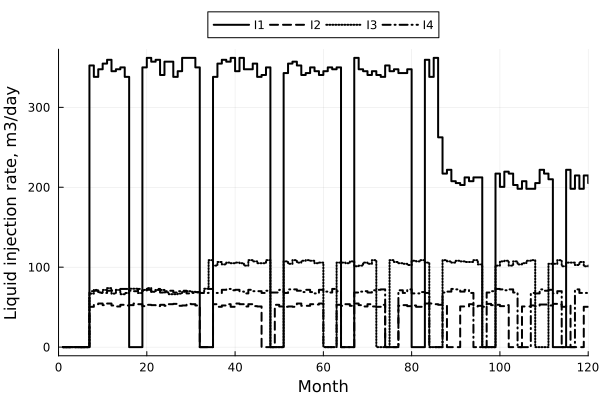
\includegraphics[height=0.65\linewidth]{fig3.png}}
      \caption{MAPE для этапов адаптации (adp) и валидации (val)}
      \label{fig:hist}
    \end{minipage} 
\end{figure}
Из рисунков видно, что модель M1 обладает наихудшими показателями как на этапе адаптации так и на этапе экзамена. Значение целевой функции примерно на порядок больше чем у остальных моделей, следовательно, модель М1 наименне пригодня для описания поведения моделируемого объета и в дальнейших исследованиях она использоваться не будет. Наилучшими характеристиками для адаптации и валидации обладает модель M3. Модели M2 и M4 имею удовлетворительные значения целевой функции. Если сравнивать только две этих модели, то M4 лучше описывает историю, а M2 - имеет лучшие прогнозные свойства, соответсвенно выбор из этих двух моделей необходимо осуществлять используюя некоторые другие критерии например такие как BIC (\cite{mus}).

На практие как правило решеется только задача адаптации и выбор модели осуществляется экспертно. Отбраковка моделей производится в основном по критерию не привышения ошибки заложенной в различных регламентах (обычно от 5 до 25\%). Соотсветсвенно модели M2-M4 ввиду сравнительно малого отличия их показателей могут быть равновероятно выбраны в качестве прогнозирующих моделей. Действительно, наиболее ярко отличие динамики давления для разных моделей наблюдается в начальный период - при вводе новых скважин и выходе на стационарные режимы работы скважин. При стационарных режимах тенденции в целом похожи, и модели при стационарных режимах имеют схожие прогнозные характеристики. 

Интересным является поведение адаптированной модели при значительном (экстремальном) изменении режима работы скважин реализованных в сценариях S1 и S2. На рисунке \ref{fig:2din} представлена динамика среднего пластового давления для трёх моделей (M2-M4) при трёх сценариях разработки (S0-S2).
\begin{figure}
\center{ 
    \begin{minipage}[h]{0.32\linewidth}
      \center{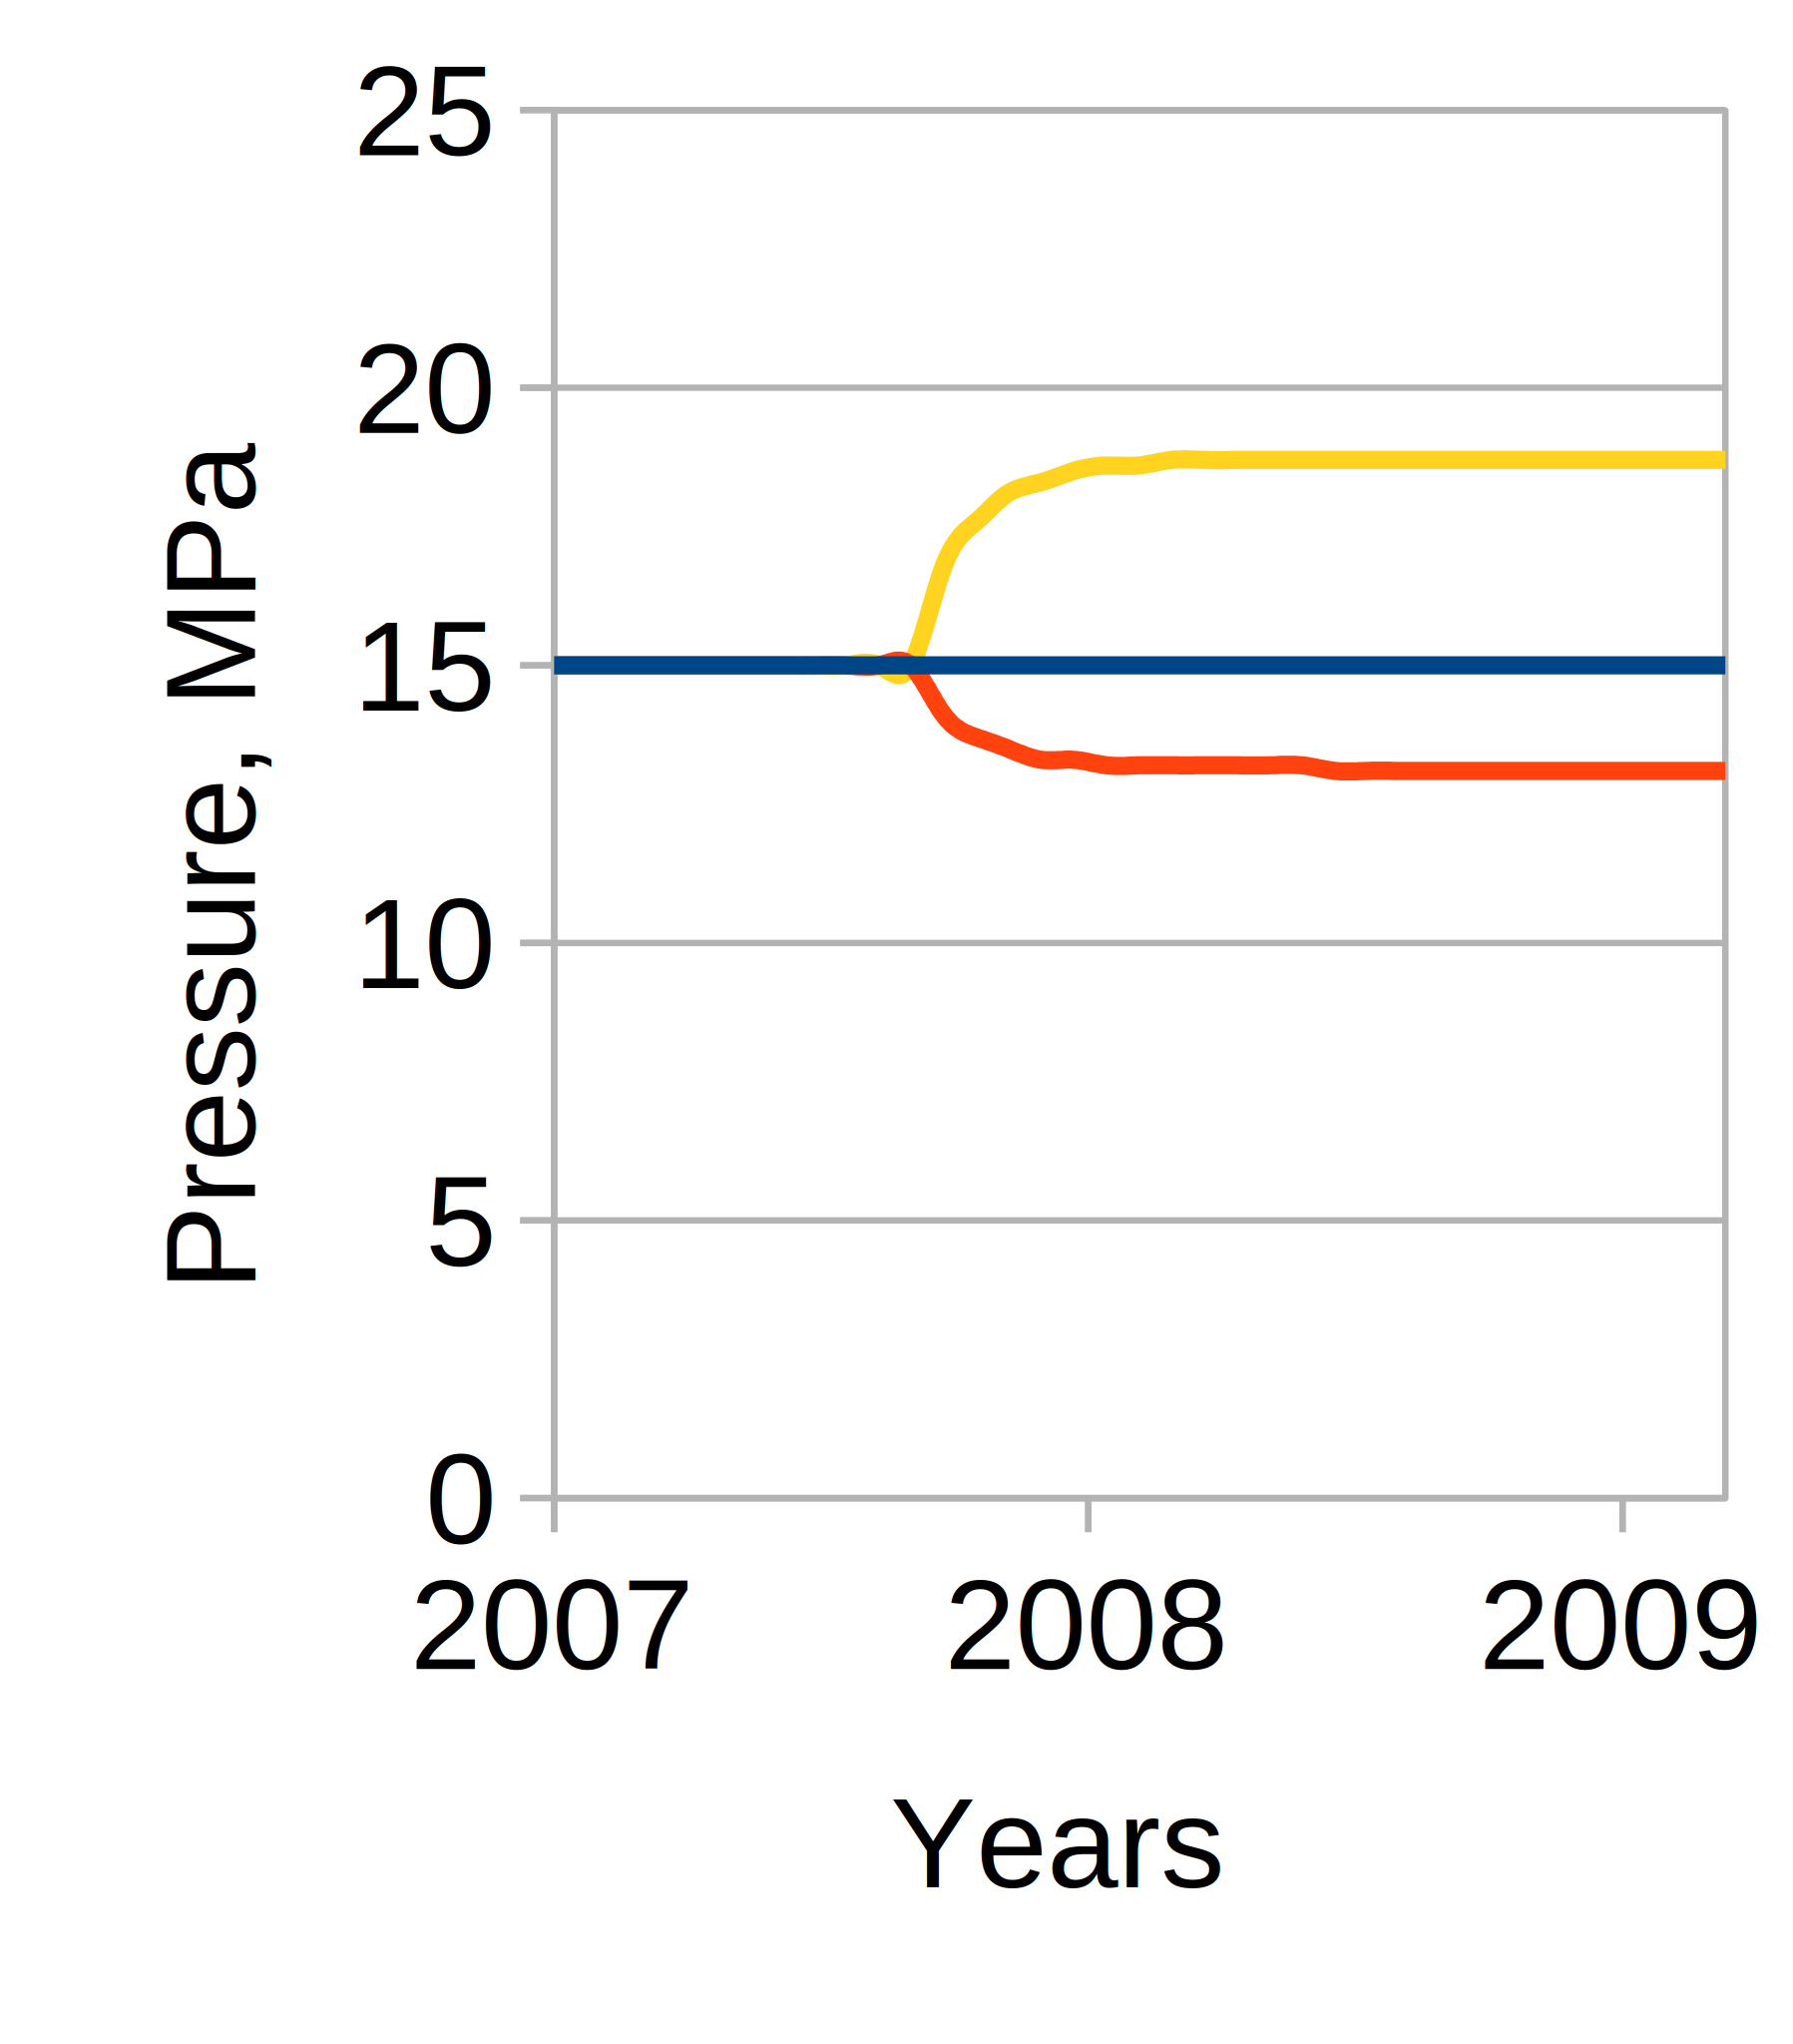
\includegraphics[height=1.5\linewidth]{fig4a.png} \\ (a)}
    \end{minipage} \hspace{0pt}
    \begin{minipage}[h]{0.32\linewidth}
      \center{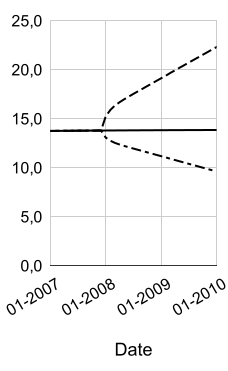
\includegraphics[height=1.5\linewidth]{fig4b.png} \\ (b)}
    \end{minipage} \hspace{0pt}
    \begin{minipage}[h]{0.32\linewidth}
      \center{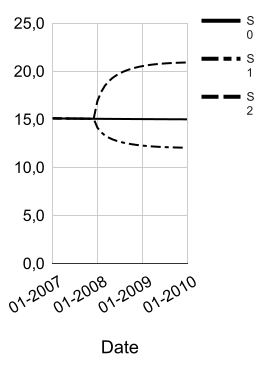
\includegraphics[height=1.5\linewidth]{fig4c.png} \\ (c)}
    \end{minipage} 
    \caption{Динамика среднего пластового давления для 3-х моделей водоносного горизонта при 3-х сценариях разработки, где a, b и c соответствуют M2, M3 и M4.}
    \label{fig:2din}
    }
\end{figure}
Как видно из графиков поведение моделей при одинаковых сценариях различны (S1 и S2). Отличие заключается не только в абсолютных значениях пластового давления, но и в динамике его изменения. Соответственно прогнозные показатели каждой модели будут существенно отличаться.

\section{CONCLUSIONS}

В результате выполненного исследования было показано, что получение удовлетворительного решения обратной задачи можно добится используя модели различной степени сложности. Помимо качества настройки модели на историю разработки - качества адаптации, также необходимо оценивать её прогнозные свойства. Проведение процедуры валидации позволяет осуществить выбор модели имеющей наилучшие прогнозные характеристики. Кроме того, в работе было продемонстрированно, что качество прогноза помимо сложности модели зависит от схожести сценариев разработки на которых адаптировалась и валидировалась модель. При  значительном отличии прогнозируемых режимов от тех на которых была осуществлена настройка модели, прогнозные свойства модели резко снижаются. По мере поступления фактических данных необходимо заново проводить процедуру структурно параметрической идентификации.

\section{FUNDING}
The study was performed by a grant from the Russian Foundation for Basic Research (project no. 18-29-10023).

%
% The Bibliography
%
\begin{thebibliography}{99}
\bibitem{mus} E.N.Musakaev, S.P.Rodionov, D.Y.Legostaev, V.P.Kosyakov,  «Parameter identification for sector filtration model of an oil reservoir with complex structure» // AIP Conference Proceedings 2125,030113 2009;

\bibitem{kos} V.P.Kosyakov, D.Y.Legostaev,  «Computational technology for solution of the reverse problem of filtration theory for oil fields with an aquifer» // AIP Conference Proceedings 2125,030112 2009;

\bibitem{bas} К.С.Басниев, Н.М.Дмитриев, Р.Д.Каневская, В.М.Максимов. Подземная гидромеханика.  М.-Ижевск: Институт компьютерных исследований, 2006. 

\bibitem{dake} L.P.Dake, Fundamentals of Reservoir Engineering (Elsevier, Amsterdam, 1978).

\bibitem{fet} M.J.Fetkovich. A Simplifi ed approach to water infl ux calculations – Finite aquifer systems. J. Pet. Tech. July 1971, vol. 23, is. 7, pp. 814–828.


\end{thebibliography}

\end{document}